\section{Передача видео}

Еще одна из важнейших проблем, решаемых WebRTC -- передача видео. Это сложный процесс, для хранения 30-минутного несжатого 720 8-битного видео требуется около 110 Гб. В таких условиях конференция с четырьмя участниками является невозможной. Для решения этой проблемы используют сжатие.

Сжатие делится на 2 типа:
\begin{itemize}
	\item[1.] Сжатие внутри кадра (intra-frame compression) -- это сжатие, которое уменьшает количество бит, используемых для описания единичного видеофрейма. Подобная техника используется для сжатия неподвижных изображений, например, JPEG;
	\item[2.] Межкадровое сжатие (inter-frame compression) -- способ не передавать одинаковую информацию дважды.
\end{itemize}

Кадры при межкадровом сжатии делятся на 3 типа:
\begin{itemize}
	\item[--] I-Frame -- полное изображение, которое может быть декодировано без каких-либо изменений;
	\item[--] P-Frame -- частичное изображение, содержащее только изменения предыдущего изображения;
        \item[--] B-Frame -- частичное изображение, представляющее собой модификацию предыдущего и последующего изображений.
\end{itemize}

Ниже приведена визуализация трех типов кадров, Рисунок ~\ref{frame-types}.

\begin{figure}[ht]
\begin{center}
\scalebox{0.15}{
   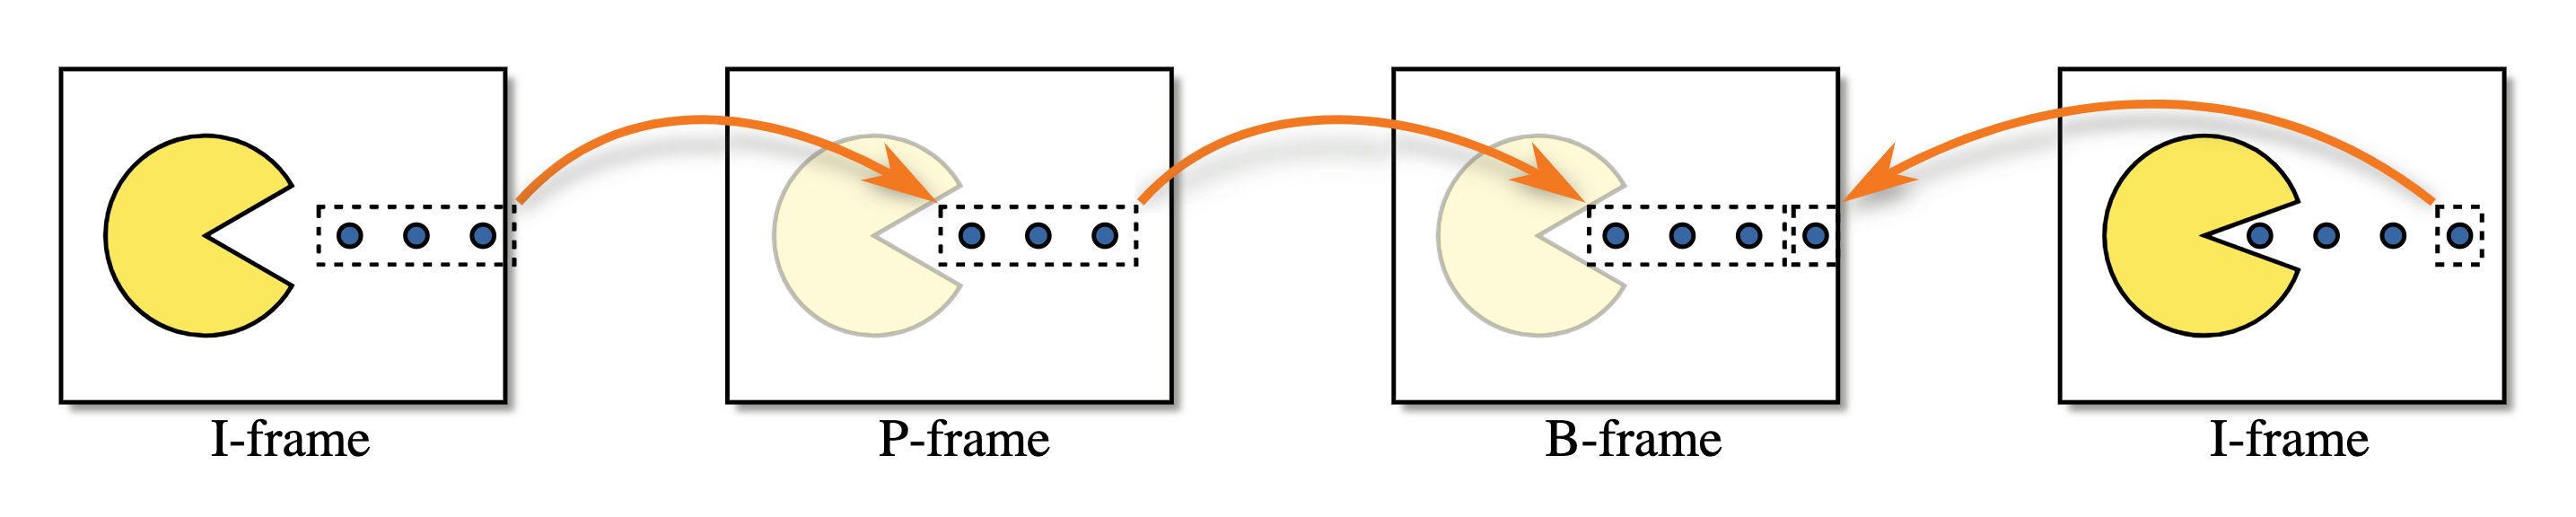
\includegraphics{images/frame_types.png}
}

\caption{
\label{frame-types}
     Типы кадров}
\end {center}
\end {figure}

\subsection{Потеря изображения}

Для решения проблемы с потерей изображения используются сообщения FIR (Full Intra Request) и PLI (Picture Loss Indication). Эти сообщения запрашивают у отправителя полный ключевой кадр.

PLI используется, когда декодер получает частичные кадры и не модет их декодировать. Такое может произойти при потере данных или ошибки декодера.

FIR не должен использоваться при потере пакетов или кадров согласно RFC 5104. FIR запрашивает ключевой кадр, например, при подключении к сессии нового участника, так как для начала декодирования видео требуется ключевой кадр, до его получения декодер будет отклонять остальные кадры \cite{v16}.

\pagebreak